\section*{Приложения}
\addcontentsline{toc}{section}{Приложения}

\subsection*{Приложение А. Гиперпараметры обучения методов.} 
\addcontentsline{toc}{subsection}{Приложение А. Гиперпараметры обучения методов.}
\label{appendix:1}

Эксперименты проводились с использованием библиотеки PyTorch \cite{pytorch} языка программирования Python 3. Применялся сторонний репозиторий с кодом, содержащий реализацию метода SimCLR \cite{simclrrepo}.

Обучение метода SimCLR велось с помощью оптимизатора Adam \cite{adam} с начальной длиной шага (англ. learning rate) $\eta=3\cdot 10^{-4}$ и коэффициентом убывания весов (англ. weight decay) $wd=10^{-4}$. При этом использовался косинусный отжиг длины шага \cite{cosine}. Другие гиперпараметры равнялись следующим значениям: размер пакета $B=256$, температура $\tau=0.07$, размерность выходного пространства $d=128$, максимальное число эпох обучения $t_{\max}=200$.

Для обучения с учителем и со случайной разметкой применялся стохастический градиентный спуск с параметром импульса $m=0.9$. Все остальные гиперпараметры обучения совпадали с методом SimCLR, кроме температуры $\tau=1$, размерности выходного пространства $d=10$ (число классов CIFAR-10) и максимального числа эпох обучения ($t_{\max}=50$ для обучения с учителем, $t_{\max}=20$ для случайной разметки и $t_{\max}=500$ для случайной разметки с аугментациями).

При обучении метода SimCLR использовались следующие аугментации:
\begin{itemize}
    \setlength\itemsep{-0.25em}
    \item вырезание случайного фрагмента изображения
    \item случайное отражение изображения по горизонтали
    \item случайное изменение яркости, контраста, насыщенности и оттенка
    \item случайная конвертация в черно-белое изображение
    \item гауссово размытие
\end{itemize}

\noindent
В случае обучения с учителем и обучения со случайной разметкой из указанных аугментаций применялось только вырезание случайного фрагмента изображения, а также поканальная нормализация изображений с вектором средних $\mu=(0.4914, 0.4822, 0.4465)$ и вектором стандартных отклонений $\sigma=(0.2023, 0.1994, 0.2010)$, характерными для набора данных CIFAR-10. На рис. \ref{appendix:pic:1} приведен фрагмент кода, уточняющий параметры использованных аугментаций.

\begin{figure}[H]
    \centering
    \renewcommand{\thefigure}{А.1}
    \setstretch{1.1}
    \begin{subfigure}[b]{0.8\textwidth}
        \centering
        \begin{lstlisting}[language=Python]
        import torchvision.transforms as T
        
        def get_simclr_transform(size):
            color_jitter = T.ColorJitter(brightness=0.8, contrast=0.8,
                                         saturation=0.8, hue=0.2)
            
            transform = T.Compose([
                T.RandomResizedCrop(size=size),
                T.RandomHorizontalFlip(),
                T.RandomApply([color_jitter], p=0.8),
                T.RandomGrayscale(p=0.2),
                T.GaussianBlur(kernel_size=int(0.1 * size)),
                T.ToTensor()
            ])
            
            return transform
        \end{lstlisting}
    \end{subfigure}
    \begin{subfigure}[b]{0.8\textwidth}
        \centering
        \begin{lstlisting}[language=Python]
        import torchvision.transforms as T
        
        def get_supervised_transform(size):
            transform = T.Compose([
                T.RandomCrop(size, padding=4),
                T.RandomHorizontalFlip(),
                T.ToTensor(),
                T.Normalize(mean=(0.4914, 0.4822, 0.4465),
                            std=(0.2023, 0.1994, 0.2010))
            ])
            
            return transform
        \end{lstlisting}
    \end{subfigure}
    \caption{Фрагмент кода на библиотеке PyTorch языка программирования Python 3, который генерирует аугментации для метода SimCLR (сверху) и для обучения с учителем (снизу).}
    \label{appendix:pic:1}
\end{figure}{}

\subsection*{Приложение Б. Дополнительные материалы экспериментов.} 
\addcontentsline{toc}{subsection}{Приложение Б. Дополнительные материалы экспериментов.}
\label{appendix:2}

Дополнительный проведенный эксперимент проверяет, что две аугментированные версии изображения в методе SimCLR имеют сопоставимые величины $r_t(x)$. Согласно рис. \ref{appendix:pic:2}, даже при рассмотрении одной пары аугментаций вероятности правильной классификации первой и второй версии изображения неплохо соотносятся, однако для некоторых изображений данные вероятности отличаются значительно. Усреднение по аугментациям нивелирует подобные объекты, уменьшая разницу в величине $r_t(x)$ между первыми и вторыми версиями изображений.

\begin{figure}[H]
    \centering
    \renewcommand{\thefigure}{Б.1}
    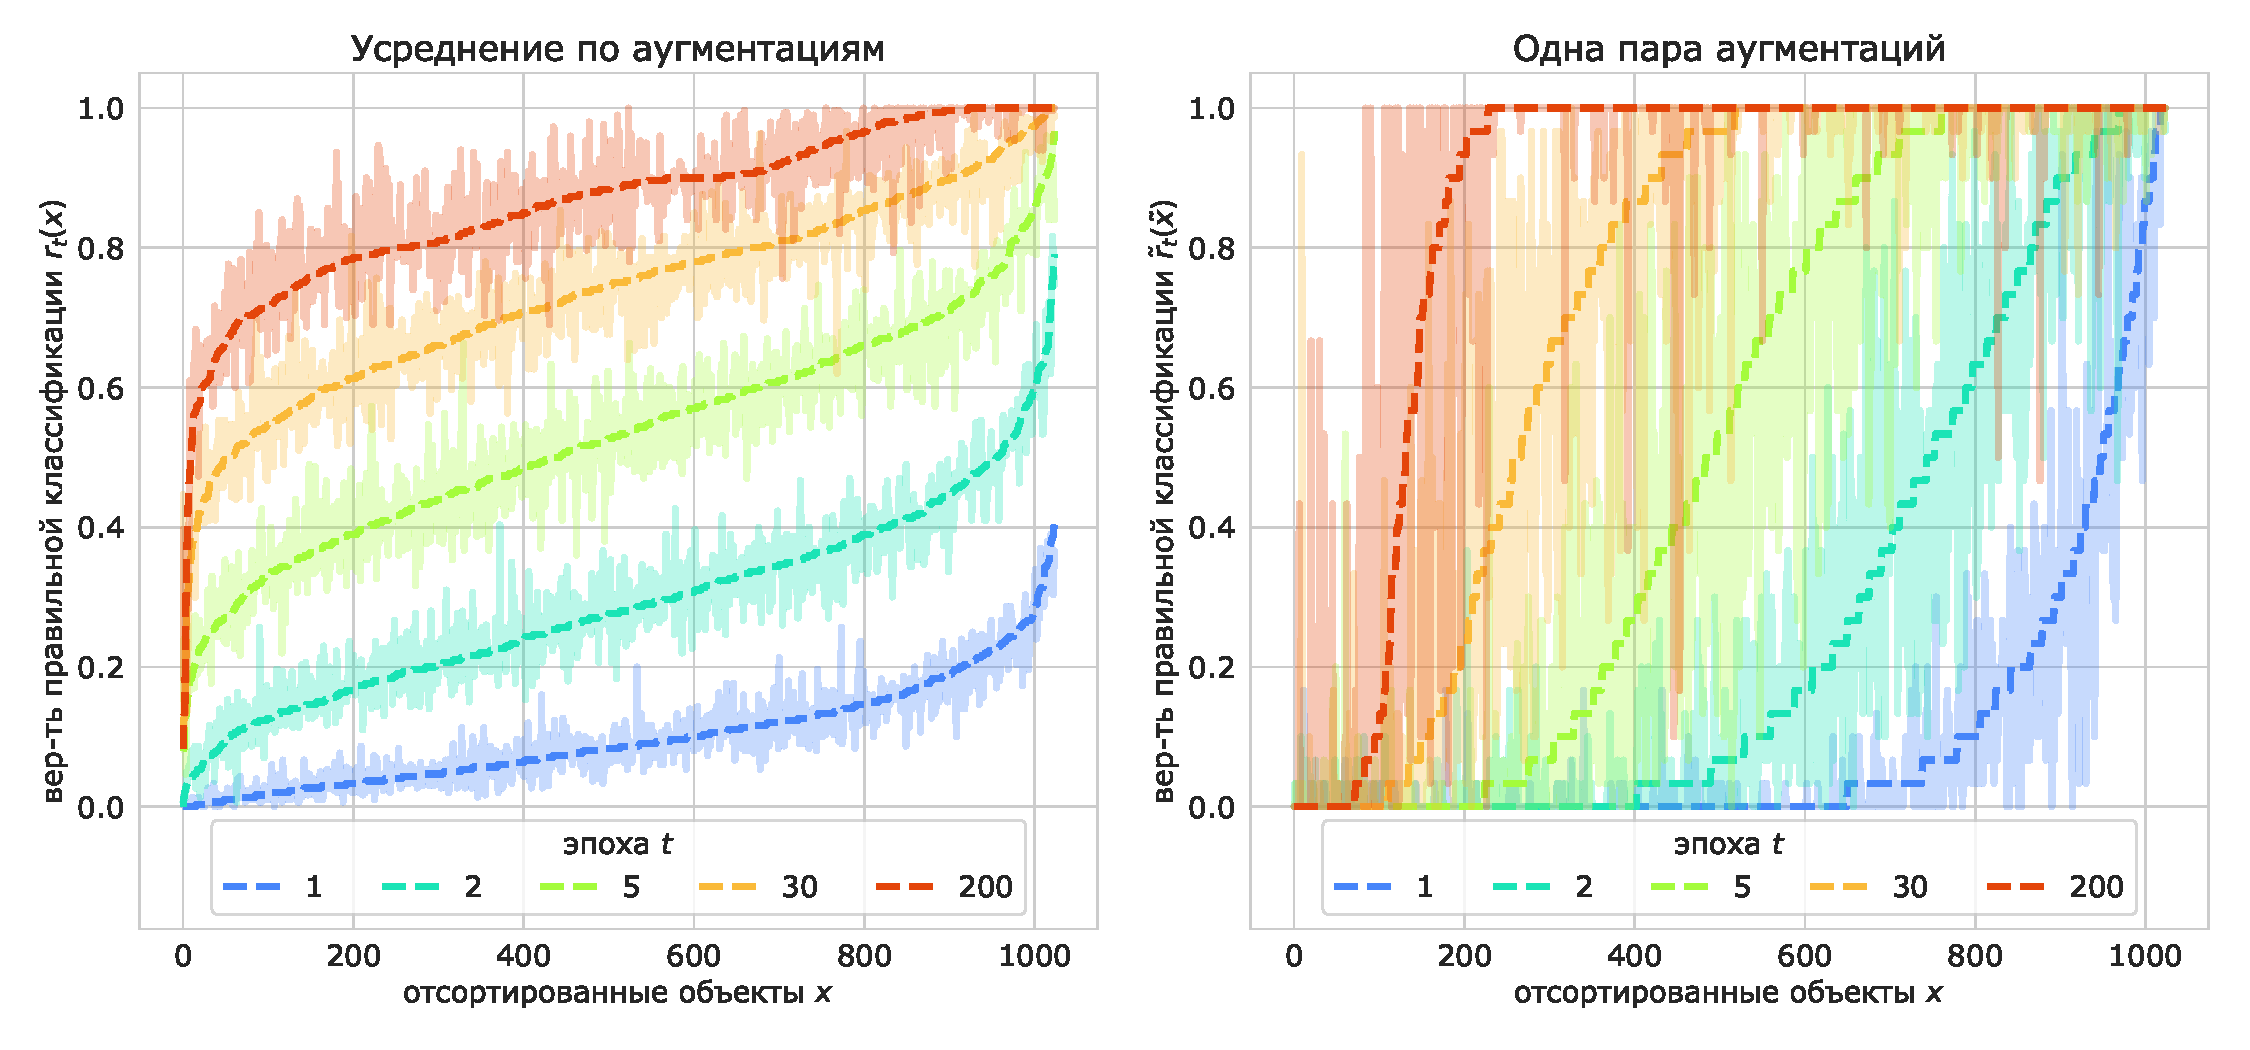
\includegraphics[width=17cm]{images/first_second.pdf}
    \caption{Сравнение величины $r_t(x)$ метода SimCLR, посчитанной по первым аугментациям изображений (пунктирная линия) и по вторым аугментациям изображений (полупрозрачная жирная линия), сортировка производится по величинам от первых аугментаций. Левый график соответствует величине $r_t(x)$, усредненной по аугментациям, а правый --- величине $\tilde{r}_t(\tilde{x})$, посчитанной по одной паре аугментаций.}
    \label{appendix:pic:2}
\end{figure}{}

Мы также проводим эксперимент, который сравнивает методы по качеству классификации на наборе данных CIFAR-10. Для этого у обученных нейронных сетей фиксируются веса, а поверх выходов предпоследнего слоя, имеющих разномерность $D=512$, обучается линейный классификатор (логистическая регресия без регуляризации). Используемый оптимизитор --- Adam с длиной шага $\eta=10^{-3}$, число эпох обучения $t=10$, размера пакета $B=256$. Помимо упомянутых в основной части методов, мы рассматриваем нейронную сеть со случайной инициализацией и обучение классификатора поверх исходных изображений. Результаты сравнения представлены в таблице \ref{appendix:tab:1}. 
\begin{table}[H]
    \centering
    \renewcommand{\thetable}{Б.1}
    \begin{tabular}{|C{5.25cm}|C{2.75cm}|C{2.75cm}|}
        \hline
         & Обучающая выборка & Тестовая выборка \\ \hline
        SimCLR \newline ($t=200$ эпох) & 0.8186	& 0.8060 \\ \hline
        Обучение с учителем \newline ($t=200$ эпох) & 1.0000 & 0.9532 \\ \hline
        Случ. разметка \newline ($t=30$ эпох) & 0.3369 & 0.3248 \\ \hline
        Случ. разметка с аугм. \newline ($t=500$ эпох) & 0.4395 & 0.4275\\ \hline
        Случ. \newline инциализация & 0.2891 & 0.2982\\ \hline
        Исходные \newline изображения & 0.4227 & 0.3768\\ \hline
    \end{tabular}
    \caption{Доля правильных ответов на наборе данных CIFAR-10 при обучении линейного классификатора поверх нейросетевых представлений.}
    \label{appendix:tab:1}
\end{table}

По доле правильных ответов закономерно выделяются обучение с учителем (как метод, который обучался непосредственно на классификацию CIFAR-10) и SimCLR (как эффективный метод предобучения). Также показательно, что случайная разметка с аугментациями имеет качество лучше, чем обычная случайная разметка, так как аугментации усложняют задачу сопоставления изображений случайным меткам и обеспечивают большую устойчивость векторных представлений. Нетривиальным результатом является то, что обе вариации обучения со случайной разметкой имеют долю правильных ответов выше, чем случайно инициализированная нейронная сеть. Данное наблюдение подтверждает, что обучение со случайной разметкой можно использовать для предобучения нейронных сетей, однако оно не выдерживает конкуренции с современными self-supervised learning методами.
